%% =====================================================================================================================
%% Manuscript source (LaTeX).  Build:  cd manuscript && pdflatex main && bibtex main && pdflatex main && pdflatex main
%% All numbers in the text are \newcommand macros written by R/07_figures_tables.R into numbers.tex; all tables are
%% generated by the same script; figures are PDFs produced by R. Nothing numerical is typed by hand in this file
%% except the static parameter/data-source tables (which mirror R/00_functions.R and are checked by tests/).
%% =====================================================================================================================
\documentclass[11pt,a4paper]{article}
\usepackage[T1]{fontenc}
\usepackage[utf8]{inputenc}
\usepackage{lmodern,microtype}
\usepackage[margin=2.4cm]{geometry}
\usepackage{amsmath,amssymb,booktabs,graphicx,xcolor,caption,enumitem,float,setspace,array}
\usepackage[numbers,sort&compress]{natbib}
\usepackage{tikz}\usetikzlibrary{arrows.meta,positioning}
\usepackage{listings}
\usepackage[mathlines]{lineno}
\usepackage[colorlinks,linkcolor=blue!50!black,citecolor=blue!50!black,urlcolor=blue!50!black]{hyperref}
% AUTO-GENERATED by R/07_figures_tables.R -- do not edit
\newcommand{\ReEightyFive}{0.89 (0.82 to 0.95)}
\newcommand{\ReEightyThree}{0.74 (0.68 to 0.79)}
\newcommand{\ReFiftyFive}{0.95 (0.86 to 1.02)}
\newcommand{\ReFiftyThree}{0.87 (0.80 to 0.93)}
\newcommand{\ReHundredFive}{0.83 (0.77 to 0.88)}
\newcommand{\ReHundredThree}{0.60 (0.55 to 0.64)}
\newcommand{\ReMedEightyFive}{0.89}
\newcommand{\ReMedEightyThree}{0.74}
\newcommand{\ReMedFiftyFive}{0.95}
\newcommand{\ReMedFiftyThree}{0.87}
\newcommand{\ReMedHundredFive}{0.83}
\newcommand{\ReMedHundredThree}{0.60}
\newcommand{\aIsoFive}{58\%}
\newcommand{\aIsoSeven}{50\%}
\newcommand{\aIsoThree}{70\%}
\newcommand{\avertEightyFive}{22,821 (5,312 to 90,341)}
\newcommand{\avertEightyThree}{27,786 (7,467 to 102,382)}
\newcommand{\avertFiftyFive}{15,595 (3,200 to 64,632)}
\newcommand{\avertFiftyThree}{23,490 (5,527 to 93,061)}
\newcommand{\avertHundredFive}{26,062 (6,700 to 98,336)}
\newcommand{\avertHundredThree}{29,088 (8,364 to 103,935)}
\newcommand{\avertedEightyFive}{22,821}
\newcommand{\avertedEightyThree}{27,786}
\newcommand{\avertedFiftyFive}{15,595}
\newcommand{\avertedFiftyThree}{23,490}
\newcommand{\avertedHundredFive}{26,062}
\newcommand{\avertedHundredThree}{29,088}
\newcommand{\baseCases}{31,089 (9,845 to 107,831)}
\newcommand{\baseCasesMed}{31,089}
\newcommand{\cfrAssumed}{48\%}
\newcommand{\critReEightyFive}{1.13}
\newcommand{\critReEightyThree}{1.36}
\newcommand{\critReFiftyFive}{1.06}
\newcommand{\critReFiftyThree}{1.15}
\newcommand{\critReHundredFive}{1.20}
\newcommand{\critReHundredThree}{1.67}
\newcommand{\crudeCFR}{48\%}
\newcommand{\deathsEightyFive}{11,023}
\newcommand{\deathsEightyThree}{13,421}
\newcommand{\deathsFiftyFive}{7,532}
\newcommand{\deathsFiftyThree}{11,346}
\newcommand{\deathsHundredFive}{12,588}
\newcommand{\deathsHundredThree}{14,050}
\newcommand{\delayHalf}{7}
\newcommand{\delayMean}{8.5}
\newcommand{\delayNinety}{15}
\newcommand{\desolveVersion}{1.40}
\newcommand{\durEightyFive}{24}
\newcommand{\durEightyThree}{9}
\newcommand{\durFiftyFive}{53}
\newcommand{\durFiftyThree}{22}
\newcommand{\durHiEightyFive}{53}
\newcommand{\durHiEightyThree}{14}
\newcommand{\durHiFiftyFive}{$>$60}
\newcommand{\durHiFiftyThree}{49}
\newcommand{\durHiHundredFive}{21}
\newcommand{\durHiHundredThree}{7}
\newcommand{\durHundredFive}{13}
\newcommand{\durHundredThree}{5}
\newcommand{\durLoEightyFive}{14}
\newcommand{\durLoEightyThree}{7}
\newcommand{\durLoFiftyFive}{21}
\newcommand{\durLoFiftyThree}{13}
\newcommand{\durLoHundredFive}{9}
\newcommand{\durLoHundredThree}{4}
\newcommand{\fitAReAfter}{1.04 (0.98 to 1.07)}
\newcommand{\fitAReAfterMed}{1.04}
\newcommand{\fitAReBefore}{1.19 (1.13 to 1.27)}
\newcommand{\fitAReBeforeMed}{1.19}
\newcommand{\fitAacf}{0.27}
\newcommand{\fitAcover}{96\%}
\newcommand{\fitAdAIC}{14.5}
\newcommand{\fitAincEnd}{63 (55 to 71)}
\newcommand{\fitAincEndMed}{63}
\newcommand{\fitApGrow}{0.95}
\newcommand{\fitArAfter}{0.004 ($-$0.001 to 0.006)}
\newcommand{\fitArBefore}{0.017 (0.011 to 0.023)}
\newcommand{\fitAtc}{5 July}
\newcommand{\fitAtcRange}{28 June to 2 August}
\newcommand{\fitBReAfter}{1.00 (0.93 to 1.06)}
\newcommand{\fitBReAfterMed}{1.00}
\newcommand{\fitBReBefore}{1.20 (1.16 to 1.25)}
\newcommand{\fitBReBeforeMed}{1.20}
\newcommand{\fitBacf}{0.01}
\newcommand{\fitBcover}{95\%}
\newcommand{\fitBdAIC}{15.4}
\newcommand{\fitBincEnd}{83 (68 to 100)}
\newcommand{\fitBincEndMed}{83}
\newcommand{\fitBpGrow}{0.56}
\newcommand{\fitBrAfter}{0.000 ($-$0.006 to 0.006)}
\newcommand{\fitBrBefore}{0.018 (0.014 to 0.022)}
\newcommand{\fitBtc}{24 July}
\newcommand{\fitBtcRange}{18 July to 7 August}
\newcommand{\fracIsoBase}{51\%}
\newcommand{\fracIsoEightyFive}{59\%}
\newcommand{\fracIsoEightyThree}{71\%}
\newcommand{\fracIsoFiftyFive}{59\%}
\newcommand{\fracIsoFiftyThree}{71\%}
\newcommand{\fracIsoHundredFive}{59\%}
\newcommand{\fracIsoHundredThree}{71\%}
\newcommand{\meanSep}{86}
\newcommand{\nConfirmed}{7,200}
\newcommand{\nDeaths}{3,475}
\newcommand{\nDraws}{1,000}
\newcommand{\nIntervals}{96}
\newcommand{\nOnsetCases}{4,724}
\newcommand{\nOnsetDays}{105}
\newcommand{\nPRCC}{1,500}
\newcommand{\nRetro}{272}
\newcommand{\nStoch}{500}
\newcommand{\nVarDraws}{300}
\newcommand{\nVariants}{17}
\newcommand{\nVintages}{55}
\newcommand{\nhIncMax}{84}
\newcommand{\nhIncMin}{81}
\newcommand{\nhRMax}{0.0009}
\newcommand{\nhRMin}{$-$0.0005}
\newcommand{\pEndBaseSixty}{0.12}
\newcommand{\pEndBaseTwentyFour}{0.01}
\newcommand{\pEndYearFiveEightyFive}{0.99}
\newcommand{\pEndYearFiveEightyThree}{1.00}
\newcommand{\pEndYearFiveFiftyFive}{0.58}
\newcommand{\pEndYearFiveFiftyThree}{0.99}
\newcommand{\pEndYearFiveHundredFive}{1.00}
\newcommand{\pEndYearFiveHundredThree}{1.00}
\newcommand{\pEndYearOneEightyFive}{0.01}
\newcommand{\pEndYearOneEightyThree}{0.90}
\newcommand{\pEndYearOneFiftyFive}{0.00}
\newcommand{\pEndYearOneFiftyThree}{0.01}
\newcommand{\pEndYearOneHundredFive}{0.33}
\newcommand{\pEndYearOneHundredThree}{1.00}
\newcommand{\pEndYearTwoEightyFive}{0.52}
\newcommand{\pEndYearTwoEightyThree}{1.00}
\newcommand{\pEndYearTwoFiftyFive}{0.05}
\newcommand{\pEndYearTwoFiftyThree}{0.60}
\newcommand{\pEndYearTwoHundredFive}{0.99}
\newcommand{\pEndYearTwoHundredThree}{1.00}
\newcommand{\pReBaseBelow}{0.44}
\newcommand{\pReBelowEightyFive}{1.00}
\newcommand{\pReBelowEightyThree}{1.00}
\newcommand{\pReBelowFiftyFive}{0.94}
\newcommand{\pReBelowFiftyThree}{1.00}
\newcommand{\pReBelowHundredFive}{1.00}
\newcommand{\pReBelowHundredThree}{1.00}
\newcommand{\pctEightyFive}{73 (55 to 84)}
\newcommand{\pctEightyThree}{89 (76 to 95)}
\newcommand{\pctFiftyFive}{50 (33 to 62)}
\newcommand{\pctFiftyThree}{75 (57 to 86)}
\newcommand{\pctHundredFive}{84 (68 to 93)}
\newcommand{\pctHundredThree}{94 (85 to 98)}
\newcommand{\pctMedEightyFive}{73\%}
\newcommand{\pctMedEightyThree}{89\%}
\newcommand{\pctMedFiftyFive}{50\%}
\newcommand{\pctMedFiftyThree}{75\%}
\newcommand{\pctMedHundredFive}{84\%}
\newcommand{\pctMedHundredThree}{94\%}
\newcommand{\popAtRisk}{4,392,200}
\newcommand{\posJun}{22.6}
\newcommand{\posSep}{17.1}
\newcommand{\prccGrowthRate}{0.42}
\newcommand{\prccInfectiousPeriod}{0.10}
\newcommand{\prccIsolationDelay}{0.94}
\newcommand{\prccIsolationEffectiveness}{$-$0.80}
\newcommand{\prccLatentPeriod}{0.27}
\newcommand{\prccStartingIncidence}{0.17}
\newcommand{\rVersion}{4.3.3 (2024-02-29)}
\newcommand{\rYear}{2024}
\newcommand{\shareOnset}{66\%}
\newcommand{\stochBase}{32,114}
\newcommand{\stochEndBase}{0.31}
\newcommand{\stochEndFive}{0.73}
\newcommand{\stochEndThree}{0.86}
\newcommand{\stochFive}{8,904}
\newcommand{\stochRatioMax}{1.09}
\newcommand{\stochRatioMin}{1.00}
\newcommand{\stochRedFive}{72\%}
\newcommand{\stochRedThree}{89\%}
\newcommand{\stochThree}{3,588}
\newcommand{\testsJun}{168}
\newcommand{\testsSep}{494}
\newcommand{\valCumMod}{10,981}
\newcommand{\valCumObs}{10,274}
\newcommand{\valErrLong}{23\%}
\newcommand{\valErrShort}{35\%}
\newcommand{\valInsideLong}{inside}
\newcommand{\valInsideShort}{outside}
\newcommand{\valModLong}{3,781}
\newcommand{\valModLongCI}{3,781 (2,796 to 4,991)}
\newcommand{\valModShort}{1,236}
\newcommand{\valNaiveErrLong}{24\%}
\newcommand{\valObsLong}{3,074}
\newcommand{\valObsShort}{916}
\newcommand{\valPredLongHi}{5,126}
\newcommand{\valPredLongLo}{2,743}
\newcommand{\valRateObsLong}{67}
\newcommand{\valRateObsShort}{61}
\newcommand{\varBaseFourFive}{$-$67 ($-$98 to $-$37)}
\newcommand{\varBaseFourThree}{80 (63 to 90)}
\newcommand{\varCondFive}{83}
\newcommand{\varCondIso}{6\%}
\newcommand{\varCondThree}{93}
\newcommand{\varErlangTenFive}{78}
\newcommand{\varErlangTenThree}{91}
\newcommand{\varErlangThreeFive}{77}
\newcommand{\varFitABase}{51,067}
\newcommand{\varFitAFive}{82}
\newcommand{\varFitAThree}{94}
\newcommand{\varFiveMax}{84}
\newcommand{\varFiveMin}{56}
\newcommand{\varGrowthHiBase}{92,275}
\newcommand{\varGrowthHiFive}{84}
\newcommand{\varGrowthHiThree}{96}
\newcommand{\varGrowthLoBase}{11,750}
\newcommand{\varGrowthLoFive}{56}
\newcommand{\varGrowthLoThree}{77}
\newcommand{\varIncHiFive}{73}
\newcommand{\varIncLoFive}{73}
\newcommand{\varPopFive}{73}
\newcommand{\varRampNinetyFive}{62}
\newcommand{\varRampNinetyThree}{81}
\newcommand{\varRampNinetyUiLo}{40}
\newcommand{\varRampThirtyFive}{69}
\newcommand{\varRampThirtyThree}{86}
\newcommand{\varThreeMax}{96}
\newcommand{\varThreeMin}{77}

\graphicspath{{../figures/}}
\captionsetup{font=small,labelfont=bf,skip=4pt}
\setlist{nosep,leftmargin=1.4em}
\onehalfspacing\setlength{\parskip}{3pt}\setlength{\parindent}{0pt}
\renewcommand{\arraystretch}{1.08}
\linenumbers\modulolinenumbers[5]
\newcommand{\Rt}{R_{\mathrm{e}}}
\newcommand{\ci}[1]{(95\%\ UI #1)}
\lstset{language=R,basicstyle=\ttfamily\fontsize{6.4}{7.4}\selectfont,breaklines=true,breakatwhitespace=false,numbers=left,numberstyle=\tiny\color{gray},
  numbersep=4pt,frame=single,rulecolor=\color{gray!50},commentstyle=\color{green!35!black}\itshape,keywordstyle=\color{blue!50!black},showstringspaces=false,
  columns=fullflexible,keepspaces=true}

\begin{document}
\thispagestyle{empty}
\begin{center}
{\LARGE\bfseries How fast is fast enough? The epidemiological benefit of shortening the symptom-onset-to-isolation delay in the 2026 Bundibugyo virus disease outbreak, Democratic Republic of the Congo: a transmission-modelling study}\\[10pt]
{\large Oluwafemi Samson Olagbami\textsuperscript{1,*}, Humphrey Rop\textsuperscript{1}, Imelda Laetitia Simboro\textsuperscript{1}, Jonathan Boakye-Yiadom\textsuperscript{1}}\\[4pt]
{\small\textsuperscript{1}Team TAUS, 2026 MPPR group modelling project (institutional affiliations to be completed by the authors)\\
\textsuperscript{*}Correspondence: olagbami.samfem@gmail.com}\\[4pt]
{\small Advisers (not authors): Dr James Azam, Andrej Jarynowski}\\[2pt]
{\small Manuscript prepared 2 November 2026 \,|\, Preliminary results \,|\, Code and data: GitHub repository accompanying this paper (URL to be inserted)}
\end{center}
\vspace{4pt}

\begin{abstract}\noindent
\textbf{Background.} The 2026 outbreak of Bundibugyo virus disease (BVD) in the Democratic Republic of the Congo (DRC) has exceeded 10\,000 confirmed cases. Every day between symptom onset and isolation is a day of possible onward transmission, yet the value of shortening that delay when isolation is imperfect has not been quantified for this outbreak.
\textbf{Methods.} We built a deterministic susceptible--exposed--infectious--isolated--removed (SEIQR) model in which the isolation rate is the inverse of the mean onset-to-isolation delay and isolated people transmit at a fraction $1-\epsilon$ of the rate of non-isolated people. We fitted it by maximum likelihood to national surveillance data up to 12 September 2026 (confirmed cases by onset date, corrected for reporting delay, and by report date), allowing one change in transmission. We simulated nine scenarios (delays of 7, 5 and 3 days $\times$ isolation effectiveness $\epsilon$ of 50\%, 80\% and 100\%) from 12 September, propagating fitted and literature uncertainty through \nDraws{} paired parameter draws, a stochastic version of the model, global and structural sensitivity analyses, and an out-of-sample forecast check.
\textbf{Findings.} Transmission grew ($\Rt\approx\fitBReBeforeMed$) until about \fitBtc{} and then plateaued ($\Rt\approx\fitBReAfterMed$); with a 7-day delay the model projected \baseCases{} symptomatic cases over 12 months (median and 95\% uncertainty interval [UI]). Reducing the mean delay to 5 days averted \pctMedFiftyFive, \pctMedEightyFive{} and \pctMedHundredFive{} of cases at 50\%, 80\% and 100\% isolation effectiveness; reducing it to 3 days averted \pctMedFiftyThree, \pctMedEightyThree{} and \pctMedHundredThree. At 80\% effectiveness, $\Rt$ fell from 1.00 to \ReMedEightyFive{} (5 days) and \ReMedEightyThree{} (3 days), and the median time to the end of transmission was \durEightyFive{} and \durEightyThree{} months, against more than 60 months at 7 days. Delay and isolation effectiveness were the dominant uncertainties (partial rank correlations \prccIsolationDelay{} and \prccIsolationEffectiveness). The benefit of a 5-day target was reversed if the true current delay were already below 5 days. A forecast made with data to 12 September overestimated the next 46 days of cases by \valErrLong.
\textbf{Interpretation.} Faster isolation can turn a plateau into decline, but quality of isolation matters as much as speed, and the size of the effect rests on the outbreak currently sitting at the epidemic threshold. Measuring the actual onset-to-isolation delay should be a surveillance priority.
\textbf{Funding.} None declared (to be confirmed by the authors).\\[3pt]
\textbf{Keywords:} Bundibugyo virus; Ebola disease; isolation; transmission model; scenario analysis; uncertainty; reproducibility
\end{abstract}

\vspace{4pt}
\noindent\fbox{\parbox{0.97\linewidth}{\small\textbf{Key points.}
\begin{itemize}
\item \textbf{Question:} how many cases would be prevented, and how much sooner would transmission end, if the mean delay from symptom onset to isolation in the DRC fell from 7 to 5 or 3 days, allowing for isolation that is only 50--100\% effective?
\item \textbf{Answer:} about \pctMedEightyFive{} (5 days) and \pctMedEightyThree{} (3 days) of the next 12 months' cases at 80\% effectiveness; \pctMedFiftyThree{} even at 50\% effectiveness with a 3-day delay.
\item \textbf{Caveats:} effects are large because the outbreak is near the threshold $\Rt\approx1$; the baseline delay is poorly measured; absolute counts are conditional on a plateau that later eased.
\end{itemize}}}
\newpage

%% ======================================================================================================================
\section{Introduction}
In May 2026 the DRC declared an outbreak of Ebola disease caused by Bundibugyo virus, which has become the second-largest Ebola-disease outbreak on record, with a crude case fatality of about \crudeCFR{} among confirmed cases \citep{zomahoun2026,kabasele2026}. By 28 October 2026, 10\,274 cases and 4\,992 deaths had been confirmed in the DRC \citep{cdcsituation2026}. Control relies on finding cases, isolating them, and tracing their contacts. Operational reviews in August found that all contact-tracing indicators were below target, that only 15--20\% of new cases were known contacts, that treatment-unit occupancy averaged 64\% (with some facilities above 100\%), and that 59\% of confirmed deaths occurred outside treatment units \citep{kabasele2026}. The delay between symptom onset and isolation is therefore a central operational quantity: community engagement, decentralised testing, rapid result return and transit centres all aim to shorten it. In the first month of the outbreak the mean delay from first symptoms to sampling was reported as 7.4 days, and a preprint from the response gives 4.6 days from onset to sampling but 8.6 days to the test result \citep{ebengo2026}.

Field teams cannot measure what a shorter delay would buy; a model can. Theory and experience from past Ebola outbreaks show that the combination of how quickly cases are isolated and how completely isolation prevents transmission determines whether an outbreak is controllable \citep{fraser2004,chowell2014,pandey2014,kucharski2015}. Scenario projections for the present outbreak have varied the \emph{fraction} of symptomatic people isolated while holding the delay fixed at two days and assuming that isolated people transmit nothing \citep{mooring2026}. To our knowledge, the benefit of shortening the delay itself, when isolation is imperfect and when the model is anchored to the observed course of this outbreak, has not been reported.

\textbf{Research question.} Among symptomatic infectious people in the DRC outbreak, how would reducing the mean onset-to-isolation delay from 7 days to 5 and 3 days change cumulative cases and outbreak duration, under worst-, base- and best-case isolation effectiveness (50\%, 80\%, 100\%)? We answer it with a transmission model fitted to surveillance data and subjected to explicit tests of its own weaknesses: reporting delay, structural assumptions about the delay distribution, an out-of-sample forecast, and a stochastic version. The analysis is fully scripted in R so that every figure, table and number in this paper can be regenerated from the data folder.

%% ======================================================================================================================
\section{Methods}
\subsection{Design, data and ethics}
This is a modelling study of publicly available, aggregated surveillance data; no individual-level data were used and no ethical approval was required (to be confirmed by the authors' institution). The scenario analysis is counterfactual: because the surveillance data end on \textbf{12 September 2026}, scenarios are applied from that date. Later official cumulative counts (27 September and 28 October) were withheld from fitting and used only for validation.

Data are the cleaned national surveillance streams compiled from the daily situation reports (SitReps) of the DRC Institut National de Sant\'e Publique (INSP) and INRB transcriptions by the BVDOutbreakSize project \citep{bvdoutbreaksize2026}, as of 12 September 2026 (\nConfirmed{} confirmed cases and \nDeaths{} confirmed deaths). Table~\ref{tab:data} lists what was used and what was not. The README of the data set warns of changing case definitions, retrospective harmonisation, a digitised onset curve and right-truncation of recent onset dates; we address each below.

\begin{table}[H]\centering\small
\caption{Data used. Streams not listed (suspected cases, bed capacity, treatment-centre movements) stop in July or August or change definition, and suspected and confirmed cases must not be mixed in one likelihood.}\label{tab:data}
\begin{tabular}{@{}p{3.5cm}p{2.7cm}p{8.3cm}@{}}\toprule
Stream & Period & Use \\\midrule
Confirmed cases by symptom-onset date (SitRep 121; 55 earlier vintages) & 25 May--6 Sep (105 days) & \textbf{Fit A}. Digitised bar chart (about 66\% of confirmed cases have a recorded onset date). The 55 vintages give the reporting-delay curve that corrects the incomplete last three weeks. \\
Cumulative confirmed cases (by report date) & 2 Jun--12 Sep (96 report intervals) & \textbf{Fit B (primary)}. Increments between report dates. The 22 July harmonisation step (369 reported, 97 new) is replaced by the printed 97, removing 272 retrospective cases. \\
Samples analysed per day & 1 Jun--12 Sep & Diagnostic only: positivity (new confirmed / samples analysed). \\
Confirmed deaths (cumulative) & 14 May--12 Sep & Crude fatality ratio for an illustrative deaths-averted figure. \\
Official cumulative confirmed cases, 27 Sep and 28 Oct & -- & Out-of-sample validation only \citep{ukhsa2026,cdcsituation2026}. \\\bottomrule
\end{tabular}\end{table}

\subsection{Model}
We use a deterministic compartmental model with susceptible ($S$), exposed ($E$), infectious but not yet isolated ($I$), isolated infectious ($Q$) and removed ($R$) people (Figure~\ref{fig:model}):
\begin{align}
\dot S &= -\lambda S, & \dot E &= \lambda S-\sigma E, & \dot I &= \sigma E-(\tau+\gamma)I, \notag\\
\dot Q &= \tau I-\gamma Q, & \dot R &= \gamma(I+Q), & \lambda &= \beta\,\frac{I+(1-\epsilon)Q}{N}, \label{eq:model}
\end{align}
where $\sigma^{-1}$ is the mean latent period, $\gamma^{-1}$ the mean infectious period (the same for isolated people), $\beta$ the transmission rate, $N$ the population at risk and $\epsilon\in[0,1]$ the \emph{isolation effectiveness}: isolated people transmit at a fraction $1-\epsilon$ of the rate of non-isolated people. The intervention is the isolation rate $\tau=1/\text{delay}$, so the mean delay studied is the mean time to isolation of a person who remains infectious and not removed. Symptomatic cases accumulate as $\dot C=\sigma E$. With $S\approx N$ the reproduction number is
\begin{equation}
\Rt=\frac{\beta}{\gamma}\left(1-\epsilon\,\frac{\tau}{\tau+\gamma}\right), \label{eq:Re}
\end{equation}
and the share of cases isolated before recovery or death is $\tau/(\tau+\gamma)$ (Appendix~\ref{app:math}). With a 7-day delay and a 7-day infectious period this share is \aIsoSeven; it is \aIsoFive{} at 5 days and \aIsoThree{} at 3 days. This competing-risk property of an exponential delay matters for interpretation and is tested by the structural analyses below.

\begin{figure}[H]\centering
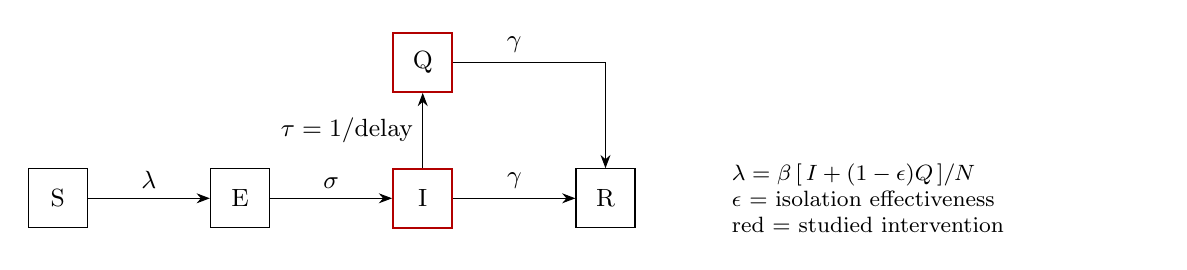
\begin{tikzpicture}[node distance=1.55cm,>=Stealth,box/.style={draw,minimum size=0.75cm,inner sep=2pt},every node/.style={font=\small}]
\node[box](S){S}; \node[box,right=of S](E){E}; \node[box,right=of E,draw=red!70!black,thick](I){I};
\node[box,right=of I](R){R}; \node[box,above=0.95cm of I,draw=red!70!black,thick](Q){Q};
\draw[->](S)--node[above]{$\lambda$}(E); \draw[->](E)--node[above]{$\sigma$}(I);
\draw[->](I)--node[above]{$\gamma$}(R); \draw[->](I)--node[left]{$\tau=1/\text{delay}$}(Q);
\draw[->](Q)-|node[above,pos=0.2]{$\gamma$}(R);
\node[right=1.1cm of R,align=left,font=\footnotesize,text width=5.3cm]{$\lambda=\beta\,[\,I+(1-\epsilon)Q\,]/N$\\ $\epsilon$ = isolation effectiveness\\ red = studied intervention};
\end{tikzpicture}
\caption{Model structure. The studied intervention is the flow from $I$ to $Q$ at rate $\tau=1/\text{delay}$; isolation is imperfect when $\epsilon<1$.}\label{fig:model}
\end{figure}

\subsection{Parameters}
Table~\ref{tab:params} gives all inputs. Natural-history values come from the model inputs of the response preprint \citep{ebengo2026} and the Ebola review of Chowell and Nishiura \citep{chowell2014}; ranges are triangular distributions that span published estimates (latent period 4.0--10.1 days, mean 6.3; infectious period 5--10 days, mean 7). We did not use the systematic-review database of Nash et al.\ \citep{nash2024}, which should replace these ranges in future work. The baseline delay of 7 days is the value in the study brief (first-month mean 7.4 days); we could not locate that figure in the primary source available to us, so two alternative baselines (4.6 and 8.6 days, the preprint's onset-to-sample and onset-to-result means) are analysed as sensitivity cases.

\begin{table}[H]\centering\small
\caption{Parameters and their sources. UI: uncertainty interval.}\label{tab:params}
\begin{tabular}{@{}p{4.1cm}p{3.6cm}p{6.6cm}@{}}\toprule
Parameter & Value & Source / treatment \\\midrule
Latent period $1/\sigma$ & triangular(4.0, 6.3, 10.1) d & \citep{ebengo2026,chowell2014}; fixed at 6.3 d in fitting, varied in scenarios \\
Infectious period $1/\gamma$ & triangular(5, 7, 10) d & \citep{ebengo2026,chowell2014}; fixed at 7 d in fitting, varied in scenarios \\
Baseline delay $1/\tau_0$ & 7 d & Study brief; 4.6 and 8.6 d in sensitivity analyses \\
Scenario delays & 7, 5, 3 d & Study design \\
Isolation effectiveness $\epsilon$ & 0.5, 0.8, 1.0 & Worst, base, best case \\
Transmission $\beta$ & estimated & Fitted (Fit B) or calibrated to the fitted growth rate in each draw \\
Starting incidence, growth rate, change date & estimated & Maximum likelihood, profile likelihood and Hessian draws \\
Count dispersion $k$ & estimated & Negative-binomial likelihood \\
Population $N$ & 4\,392\,200 & Ituri province (scalars file); depletion negligible, 10 million tested \\
Crude fatality ratio & \cfrAssumed{} & 3\,475 / 7\,200 confirmed at 12 Sep; an upper bound, used only for illustration \\
Horizon & 12 months (cases); 60 months (duration) & Study design \\\bottomrule
\end{tabular}\end{table}

\subsection{Fitting}
\textbf{Reporting delay.} The onset curve is published in every SitRep, so each onset date's count is observed repeatedly as reports accumulate. We measured the share $c(L)$ of an onset day's final count already visible $L$ days later, pooling the \nVintages{} vintages and taking counts at least 28 days old in the latest vintage as final. A Weibull cumulative distribution, $c(L)=1-\exp\{-((L+0.5)/s)^{\kappa}\}$, was fitted by least squares. Half of cases were visible after \delayHalf{} days and 90\% after \delayNinety{} days (mean \delayMean{} days).

\textbf{Observation model and likelihood.} Counts $y$ are negative-binomial with mean $\mu$ and variance $\mu+\mu^2/k$. In Fit A (onset curve) $\mu_d=c(L_d)\,i(d)$, where $i(d)$ is the model's symptomatic incidence on day $d$ and $L_d$ the days between $d$ and the report date of 12 September. In Fit B (report date) the expected increment over a report interval is the sum, over its days $u$, of $\sum_{d\le u} i(d)\{c(u-d)-c(u-d-1)\}$, i.e.\ incidence convolved with the same delay. Fit B is the primary fit because it covers all confirmed cases and is not affected by truncation; Fit A is the cross-check.

\textbf{Parameters estimated.} Natural-history parameters and the baseline delay are fixed at their central values; we estimate the starting incidence $i_0$, the transmission rate before ($\beta_1$) and after ($\beta_2$) a change on date $t_c$, and $k$. We compared this with constant transmission by AIC (counting $t_c$ as a parameter). Optimisation used Nelder--Mead from multiple stages; the date $t_c$ was profiled on a grid (5-day steps, refined to 1 day). Uncertainty draws sample $t_c$ with weights proportional to the profile likelihood and the other parameters from the multivariate normal given by the Hessian at that $t_c$. Model adequacy was checked by 95\% predictive coverage and residual autocorrelation, and by refitting at extreme natural-history values.

\subsection{Scenarios, outcomes and uncertainty propagation}
Each of \nDraws{} draws contains the fitted post-change growth rate $r$ and incidence on 12 September $i(T)$ (jointly, from Fit B), and latent and infectious periods drawn independently from their triangular distributions. For each draw and each $\epsilon$, $\beta$ is solved so that the 7-day baseline has growth rate $r$ (the dominant eigenvalue of the linearised $(E,I,Q)$ system), the initial state is the corresponding eigenvector scaled to $i(T)$, and the three delays are then simulated by changing only $\tau$. All nine scenarios share the same draws, so cases averted are within-draw differences from the 7-day run with the same $\epsilon$. This choice means that $\beta$, and therefore $\epsilon$, are not separately identifiable from case counts: $\epsilon$ is a scenario assumption.

\textbf{Outcomes.} \emph{Primary:} cumulative symptomatic confirmed cases over the next 12 months, cases averted (absolute and percentage), and outbreak duration, defined as the first day with fewer than one exposed or infectious person within 60 months (otherwise right-censored; we report medians with censoring, and the probability of ending by 12, 24 and 60 months). \emph{Secondary:} $\Rt$, probability $\Rt<1$, peak incidence and time to peak. Deaths averted are illustrative only (cases averted $\times$ \cfrAssumed). Results are medians with 95\% UIs (2.5th--97.5th percentiles). A policy surface (delays of 2--10 days, $\epsilon$ of 30--100\%; 100 draws) gives the continuous picture.

\subsection{Stochastic model}
A discrete-time binomial-chain version ($\Delta t=0.25$ d, same transitions as Eq.~\ref{eq:model}) was run for \nStoch{} replicates per scenario, each with its own parameter draw. Transmission was calibrated in discrete time so that the expected growth rate equals the deterministic one (an uncorrected calibration biased results upwards in a preliminary run).

\subsection{Sensitivity and structural analyses}
\textbf{Global:} partial rank correlation coefficients (PRCC) \citep{blower1994,marino2008} for 12-month cases over \nPRCC{} samples of latent period, infectious period, growth rate, starting incidence, $\epsilon\sim U(0.5,1)$ and delay $\sim U(3,7)$ days, with 300 bootstrap resamples for intervals. \textbf{Variants} (\nVariants{} analyses at $\epsilon=0.8$, \nVarDraws{} draws each): extreme natural-history values; growth rate and starting incidence at their 2.5th and 97.5th percentiles; fitting to the onset curve instead; true baseline delay of 4.6 or 8.6 days; Erlang-distributed delay with 3 or 10 stages (less variable delays \citep{lloyd2001}); delay defined as the mean time to isolation \emph{among those isolated} ($\tau=1/D-\gamma$); a population of 10 million; and implementation ramp-up over 30 or 90 days.

\subsection{Out-of-sample validation}
Using only data to 12 September, we forecast confirmed cases reported by 27 September and 28 October (baseline: nothing changes) and compared them with the official cumulative counts \citep{ukhsa2026,cdcsituation2026}, together with a benchmark of constant incidence equal to the mean of the last 14 days.

\subsection{Software and reproducibility}
Everything was run in R \rVersion{} with the \texttt{deSolve} package (version \desolveVersion) \citep{rcore,desolve2010}; base R provides optimisation, random numbers and graphics. All random seeds are fixed. Eight scripts (\texttt{R/00\_functions.R} to \texttt{R/07\_figures\_tables.R}) run in order from \texttt{R/run\_all.R}; \texttt{tests/test\_model.R} checks the code against analytic results (e.g.\ $\Rt=1$ exactly when the growth rate is zero; stochastic mean within 5\% of the deterministic solution). The scripts write every table, figure and in-text number (as \LaTeX{} macros) used here. The code is listed in Appendix~D and the repository README gives run times and the directory layout (Appendix~C).

%% ======================================================================================================================
\section{Results}
\subsection{Surveillance data and model fit}
Confirmed cases per day rose from about 35--40 in early June to a plateau of about 80 per day from late July (Figure~\ref{fig:fit}). Reports of onset dates reach their final value slowly: the fitted reporting delay has a mean of \delayMean{} days, so the apparent fall in the last three weeks of the onset curve is a reporting artefact, which the fitted model reproduces (Figure~\ref{fig:fit}b). A change in transmission was strongly supported in both datasets (Table~\ref{tab:fit}): $\Delta$AIC against constant transmission was \fitAdAIC{} (onset curve) and \fitBdAIC{} (report date). Growth was \fitBrBefore{} per day before about \fitBtc{} (95\% profile interval \fitBtcRange) and \fitBrAfter{} per day afterwards in Fit B, corresponding to $\Rt$ of \fitBReBefore{} before and \fitBReAfter{} after. Fit A agreed (change about \fitAtc, interval \fitAtcRange; growth after \fitArAfter; $\Rt$ \fitAReAfter). The model's incidence on 12 September was \fitBincEnd{} cases per day (Fit B) or \fitAincEnd{} (Fit A, which covers only cases with a recorded onset date, about \shareOnset{} of confirmed cases).

\begin{table}[H]\centering\scriptsize
\caption{Fitted parameters (median and 95\% uncertainty interval of draws combining the profile over the change date and the Hessian approximation), with isolation effectiveness 80\% and baseline delay 7 days. Growth rates are per day. Fits for 50\% and 100\% give the same growth rates (Appendix Table~\ref{tab:byeff}).}\label{tab:fit}
\resizebox{\textwidth}{!}{\begin{tabular}{@{}lccccccc@{}}
\toprule
Fit & Growth rate before (/d) & Growth rate after (/d) & $R_e$ before & $R_e$ after & Change date (95\% interval) & $\Delta$AIC & Incidence 12 Sep (/d) \\
\midrule
A: onset curve & 0.0169 (0.0112--0.0234) & 0.0040 ($-$0.0015 to 0.0065) & 1.19 (1.13--1.27) & 1.04 (0.98--1.07) & 5 July (28 June--2 August) & 14.5 & 63 (55--71) \\
B: report date & 0.0177 (0.0140--0.0216) & 0.0004 ($-$0.0062 to 0.0058) & 1.20 (1.16--1.25) & 1.00 (0.93--1.06) & 24 July (18 July--7 August) & 15.4 & 83 (68--100) \\
\bottomrule
\end{tabular}
}\end{table}

\begin{figure}[H]\centering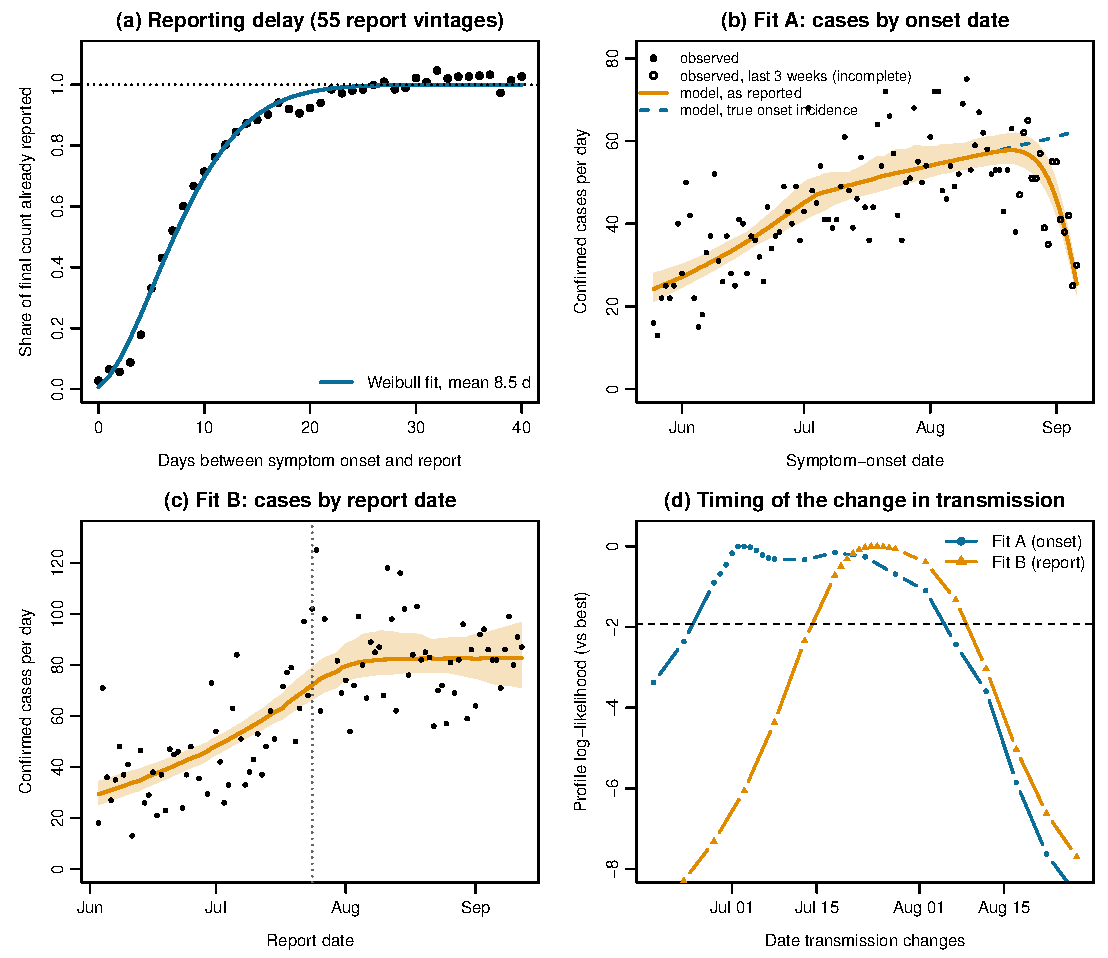
\includegraphics[width=0.98\textwidth]{fig2_fit.pdf}
\caption{Model fit. (a) Reporting delay measured from 55 SitRep vintages. (b) Fit A: confirmed cases by onset date; open circles are the incomplete last three weeks; orange is the model as it would be reported, blue dashed the true onset incidence it implies. (c) Fit B: confirmed cases per day by report date (22 July step removed); dotted line marks the estimated change date. (d) Profile log-likelihood for the date of the change in transmission (dashed line: 95\% limit).}\label{fig:fit}\end{figure}

Both fits were adequate: 95\% negative-binomial predictive intervals covered \fitAcover{} (Fit A) and \fitBcover{} (Fit B) of observations, with lag-1 residual autocorrelation of \fitAacf{} and \fitBacf. Refitting Fit B at the four extreme corners of the natural-history ranges changed the post-change growth rate only between \nhRMin{} and \nhRMax{} per day and the 12 September incidence between \nhIncMin{} and \nhIncMax{} (Appendix Table~\ref{tab:nh}), which supports using these two quantities as data-determined inputs to the scenarios. Over the same period testing expanded from \testsJun{} to \testsSep{} samples per day and positivity fell from \posJun\% to \posSep\% (Appendix Table~\ref{tab:pos}): confirmed counts grew much more slowly than testing, so the plateau is unlikely to be purely a laboratory-capacity artefact, although the data cannot show whether true incidence was flat or falling.

\subsection{Baseline: a 7-day delay}
With the delay unchanged the model projects a plateau: median $\Rt$ 1.00, with a proportion \pReBaseBelow{} of draws below 1, and \baseCases{} symptomatic cases in the next 12 months (median and 95\% UI). The interval is wide because the uncertainty in the growth rate (about $\pm0.006$ per day) compounds over a year. Transmission had ended within five years in only a proportion \pEndBaseSixty{} of draws; in the remainder it persisted.

\subsection{Scenarios}
Shortening the delay converted the plateau into decline in all eight alternative scenarios (Table~\ref{tab:scen}, Figures~\ref{fig:traj} and~\ref{fig:avert}). At 80\% effectiveness, a 5-day delay averted \pctMedEightyFive{} of cases ($\approx$\avertedEightyFive{} cases) and a 3-day delay averted \pctMedEightyThree{} (\avertedEightyThree{} cases). The corresponding $\Rt$ were \ReEightyFive{} and \ReEightyThree. At 50\% effectiveness the benefit was smaller but still substantial (\pctMedFiftyFive{} for 5 days; \pctMedFiftyThree{} for 3 days), and at 100\% it was \pctMedHundredFive{} and \pctMedHundredThree. Illustratively, applying the crude fatality ratio of \cfrAssumed, the 3-day scenario at 80\% effectiveness corresponds to about \deathsEightyThree{} fewer deaths.

\begin{table}[H]\centering\scriptsize
\caption{Scenario results from 12 September 2026 (median and 95\% UI over \nDraws{} paired draws). Months to end: first day with fewer than one exposed or infectious person; $>$60 means not ended within five years in at least half of draws. $^\dagger$Cases averted $\times$ \cfrAssumed; illustrative upper bound.}\label{tab:scen}
\resizebox{\textwidth}{!}{\begin{tabular}{@{}rrcrrrrr@{}}
\toprule
Isolation & Delay & $R_e$ & Cases in 12 months & Cases averted (\%) & Deaths averted$^\dagger$ & Months to end & P(ended $\le$24 mo) \\
effectiveness & (days) & median (95\% UI) & median (95\% UI) & median (95\% UI) & median & median (95\% UI) &  \\
\midrule
50\% & 7 & 1.00 (0.92--1.08) & 31,201 (9,854--109,025) & -- & -- & $>$60 & 0.01 \\
 & 5 & 0.95 (0.86--1.02) & 15,405 (6,232--44,057) & 50 (33--62) & 7,532 & 53 (21 to $>$60) & 0.05 \\
 & 3 & 0.87 (0.80--0.93) & 7,695 (4,033--16,443) & 75 (57--86) & 11,346 & 22 (13 to 49) & 0.60 \\
\midrule
80\% & 7 & 1.00 (0.92--1.07) & 31,089 (9,845--107,831) & -- & -- & $>$60 & 0.01 \\
 & 5 & 0.89 (0.82--0.95) & 8,212 (4,127--18,244) & 73 (55--84) & 11,023 & 24 (14 to 53) & 0.52 \\
 & 3 & 0.74 (0.68--0.79) & 3,313 (2,133--5,309) & 89 (76--95) & 13,421 & 9 (7 to 14) & 1.00 \\
\midrule
100\% & 7 & 1.00 (0.93--1.06) & 30,961 (9,833--106,530) & -- & -- & $>$60 & 0.01 \\
 & 5 & 0.83 (0.77--0.88) & 4,807 (2,779--8,746) & 84 (68--93) & 12,588 & 13 (9 to 21) & 0.99 \\
 & 3 & 0.60 (0.55--0.64) & 1,817 (1,234--2,728) & 94 (85--98) & 14,050 & 5 (4 to 7) & 1.00 \\
\bottomrule
\end{tabular}
}\end{table}

Time to the end of transmission was even more sensitive to the delay than cases. At 80\% effectiveness the median was \durEightyThree{} months (UI \durLoEightyThree--\durHiEightyThree) at 3 days against \durEightyFive{} months (\durLoEightyFive--\durHiEightyFive) at 5 days and more than 60 months at 7 days (Figure~\ref{fig:avert}b). With only 50\% effectiveness a 3-day delay still ended transmission in a median of \durFiftyThree{} months, whereas a 5-day delay needed \durFiftyFive{} months (UI \durLoFiftyFive{} to \durHiFiftyFive). The probability that transmission had ended within two years was \pEndYearTwoEightyThree{} (3 days) and \pEndYearTwoEightyFive{} (5 days) at 80\% effectiveness, and \pEndYearTwoFiftyThree{} and \pEndYearTwoFiftyFive{} at 50\%.

\begin{figure}[H]\centering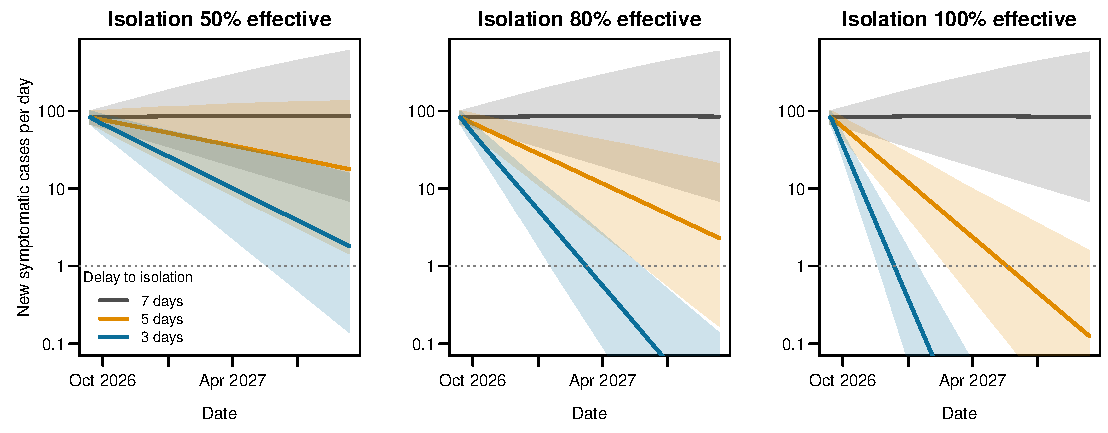
\includegraphics[width=\textwidth]{fig3_trajectories.pdf}
\caption{Projected new symptomatic cases per day from 12 September 2026 for the three delays (median and 95\% UI; logarithmic scale; dotted line: one case per day) at each isolation effectiveness.}\label{fig:traj}\end{figure}

\begin{figure}[H]\centering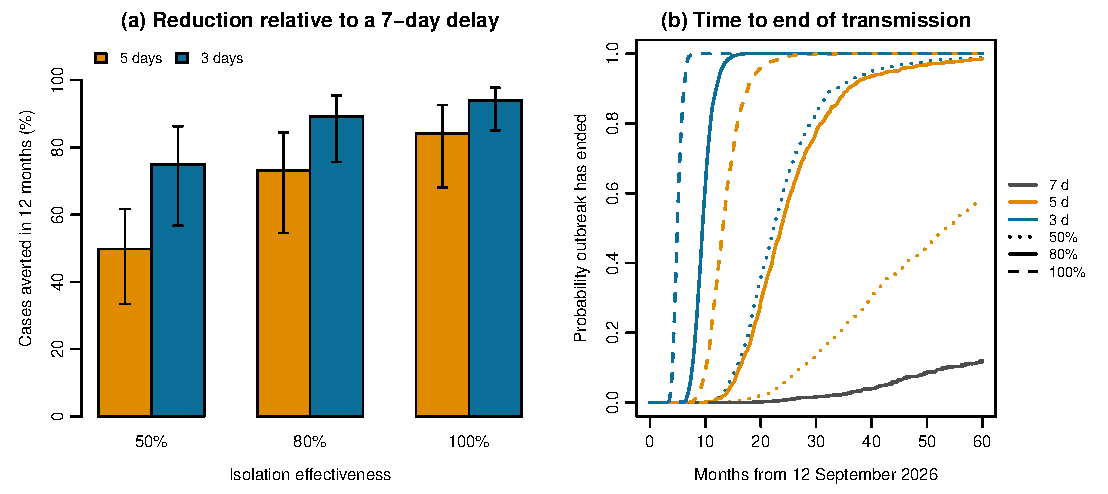
\includegraphics[width=\textwidth]{fig4_averted_duration.pdf}
\caption{(a) Percentage of 12-month cases averted relative to the 7-day delay with the same isolation effectiveness (median, 95\% UI). (b) Probability that transmission has ended, by months from 12 September 2026, for the nine scenarios (colour: delay; line type: effectiveness).}\label{fig:avert}\end{figure}

The continuous surface (Figure~\ref{fig:surf}) shows diminishing returns: at 80\% effectiveness the first two days gained (7 to 5) averted \pctMedEightyFive{} and the next two (5 to 3) a further 16 percentage points, and delays above 7 days increase cases steeply. Because the baseline sits at the threshold, the white contour (half of draws with $\Rt<1$) lies at the 7-day delay itself.

\begin{figure}[H]\centering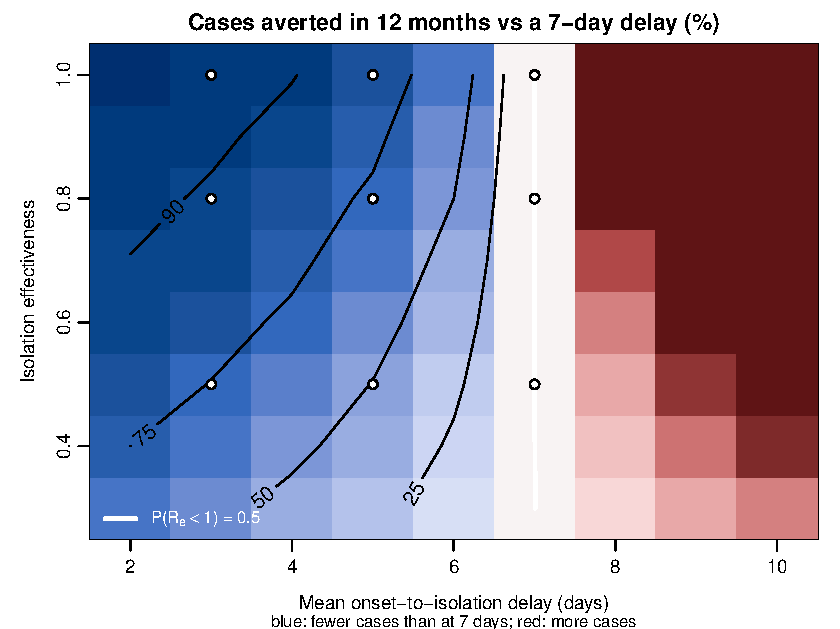
\includegraphics[width=0.7\textwidth]{fig5_policy_surface.pdf}
\caption{Policy surface: median percentage of 12-month cases averted relative to a 7-day delay, by delay and isolation effectiveness (100 draws per cell). Circles mark the nine scenarios; the white line marks where half of draws have $\Rt<1$.}\label{fig:surf}\end{figure}

\subsection{Stochastic check}
The stochastic model reproduced the deterministic medians (ratio \stochRatioMin{} to \stochRatioMax{} across scenarios; Table~\ref{tab:stoch}, Figure~\ref{fig:stoch}). At 80\% effectiveness, median cases fell from \stochBase{} (7 days) to \stochFive{} (5 days) and \stochThree{} (3 days), reductions of \stochRedFive{} and \stochRedThree. Chance events made early extinction more likely than in the deterministic model: the probability of ending within five years at 7 days was \stochEndBase{} (deterministic \pEndBaseSixty), and within two years at 5 days \stochEndFive{} (deterministic \pEndYearTwoEightyFive{}). The conclusions are therefore robust to demographic stochasticity.

\begin{table}[H]\centering\scriptsize
\caption{Stochastic (500 replicates) and deterministic results by scenario.}\label{tab:stoch}
\resizebox{\textwidth}{!}{\begin{tabular}{@{}rrcccccc@{}}
\toprule
Isolation & Delay & Stochastic cases & Deterministic & P(ended $\le$12 mo) & P(ended $\le$24 mo) & P(ended $\le$60 mo) & Deterministic \\
effectiveness & (days) & median (95\% range) & median & & & & P($\le$60 mo) \\
\midrule
50\% & 7 & 31,982 (8,450--107,440) & 31,554 & 0.00 & 0.14 & 0.27 & 0.12 \\
 & 5 & 16,508 (5,864--46,870) & 15,776 & 0.00 & 0.27 & 0.71 & 0.56 \\
 & 3 & 8,528 (3,956--19,595) & 7,822 & 0.08 & 0.71 & 0.99 & 0.99 \\
\midrule
80\% & 7 & 32,114 (8,623--110,110) & 31,391 & 0.00 & 0.14 & 0.31 & 0.12 \\
 & 5 & 8,904 (4,071--19,945) & 8,281 & 0.10 & 0.73 & 0.99 & 0.98 \\
 & 3 & 3,588 (2,173--5,772) & 3,313 & 0.86 & 1.00 & 1.00 & 1.00 \\
\midrule
100\% & 7 & 31,062 (8,615--107,137) & 31,147 & 0.01 & 0.16 & 0.36 & 0.12 \\
 & 5 & 5,055 (2,731--9,547) & 4,792 & 0.61 & 1.00 & 1.00 & 1.00 \\
 & 3 & 1,914 (1,279--2,893) & 1,815 & 1.00 & 1.00 & 1.00 & 1.00 \\
\bottomrule
\end{tabular}
}\end{table}
\begin{figure}[H]\centering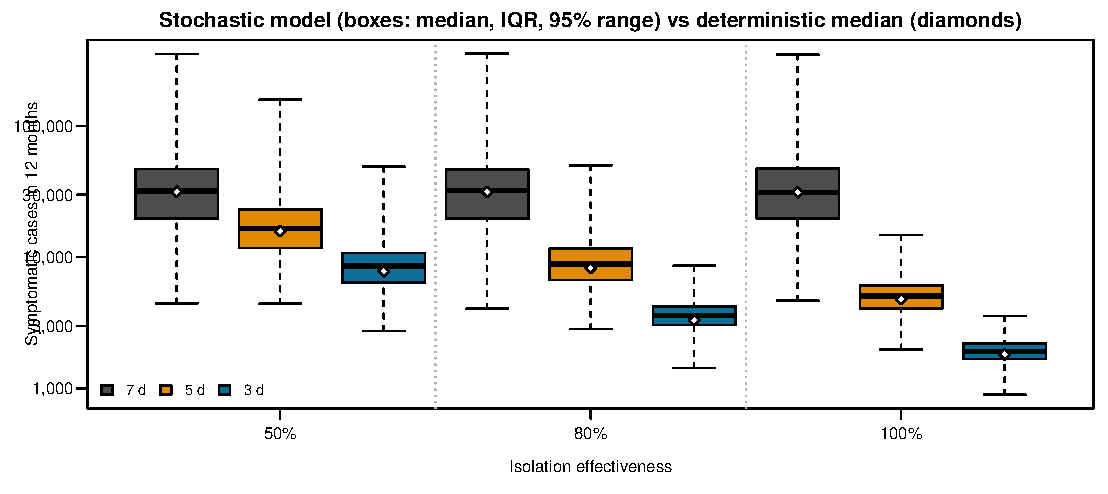
\includegraphics[width=0.95\textwidth]{fig7_stochastic.pdf}
\caption{Stochastic distribution of 12-month cases (boxes: median and interquartile range; whiskers: 95\% range) with the deterministic median (diamonds).}\label{fig:stoch}\end{figure}

\subsection{Sensitivity analyses}
In the global analysis (Figure~\ref{fig:sens}a; Appendix Table~\ref{tab:prcc}) the isolation delay had the largest influence on 12-month cases (PRCC \prccIsolationDelay), followed by isolation effectiveness (\prccIsolationEffectiveness), baseline growth rate (\prccGrowthRate), latent period (\prccLatentPeriod), starting incidence (\prccStartingIncidence) and infectious period (\prccInfectiousPeriod). In the structural and assumption analyses (Figure~\ref{fig:sens}b; Table~\ref{tab:var}), percentage reductions at 80\% effectiveness ranged from \varFiveMin{} to \varFiveMax\% for a 5-day delay and \varThreeMin{} to \varThreeMax\% for a 3-day delay, with one exception. Percentages were almost unchanged across the 95\% range of starting incidence (\varIncLoFive{} to \varIncHiFive\% for 5 days), although absolute counts scaled with it. Reductions were larger with less variable delays (Erlang-3: \varErlangThreeFive\%; Erlang-10: \varErlangTenFive\% at 5 days), and also when the delay was defined among isolated cases (\varCondFive\% and \varCondThree\%), because in that reading the 7-day baseline isolates only \varCondIso{} of cases. They were smaller when interventions took 30 or 90 days to reach full effect (\varRampThirtyFive\% and \varRampNinetyFive\% for 5 days; \varRampThirtyThree\% and \varRampNinetyThree\% for 3 days), and were insensitive to population size (\varPopFive\%). Fitting to the onset curve gave \varFitAFive\% and \varFitAThree\% but a larger baseline case count (\varFitABase) because its post-change growth was slightly positive. The baseline growth rate was the main source of spread in the baseline projection, ranging from \varGrowthLoBase{} to \varGrowthHiBase{} cases across its 95\% range, while the percentage averted moved from \varGrowthLoFive{} to \varGrowthHiFive\% (5 days).

\textbf{The exception is the baseline delay.} If the true current mean delay were already 4.6 days (the preprint's onset-to-sample mean), a ``5-day'' policy would be \emph{worse} than the status quo: cases would rise (percentage averted: \varBaseFourFive), while a 3-day target would still avert \varBaseFourThree{} percent. If the current delay were 8.6 days, the gains would be larger (5 days: 82\%; 3 days: 91\%). Hence the 7-day baseline must be verified.

\begin{figure}[H]\centering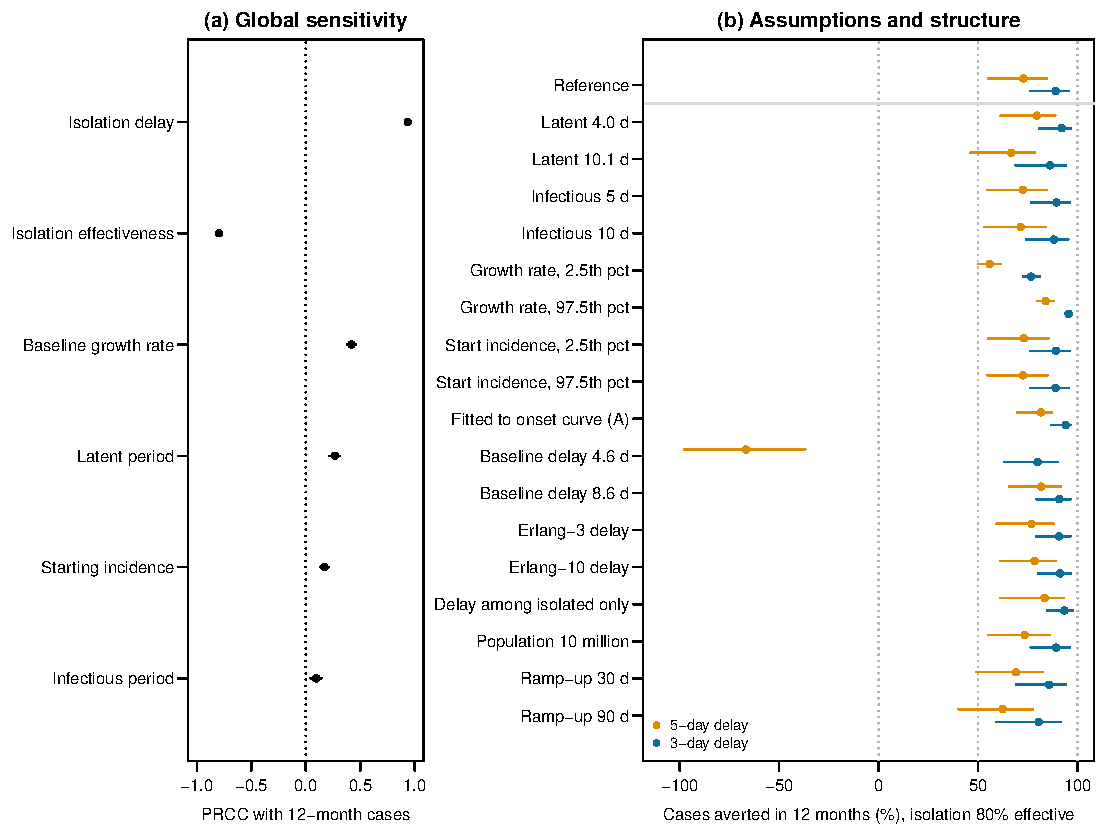
\includegraphics[width=\textwidth]{fig6_sensitivity.pdf}
\caption{(a) PRCC (with 95\% bootstrap CI) of 12-month cases against each parameter. (b) Percentage of 12-month cases averted at 80\% effectiveness under each assumption (median and 95\% UI), for 5-day and 3-day delays.}\label{fig:sens}\end{figure}

\begin{table}[H]\centering\scriptsize
\caption{Assumption and structure analyses at 80\% isolation effectiveness: percentage of 12-month cases averted vs the (variant-specific) baseline delay; median (95\% UI) over \nVarDraws{} draws.}\label{tab:var}
\begin{tabular}{@{}lccc@{}}
\toprule
Variant & 5-day delay (\%) & 3-day delay (\%) & $R_e$ at 3 d \\
\midrule
Reference (all uncertainty propagated) & 73 (55 to 85) & 89 (76 to 96) & 0.74 \\
\multicolumn{4}{@{}l}{\textit{Natural history}} \\
\quad Latent period 4.0 d & 79 (61 to 89) & 92 (81 to 97) & 0.74 \\
\quad Latent period 10.1 d & 67 (46 to 79) & 86 (69 to 94) & 0.74 \\
\quad Infectious period 5 d & 73 (54 to 85) & 89 (77 to 96) & 0.75 \\
\quad Infectious period 10 d & 72 (53 to 84) & 88 (74 to 95) & 0.73 \\
\multicolumn{4}{@{}l}{\textit{Calibration}} \\
\quad Growth rate at 2.5th percentile & 56 (50 to 62) & 77 (73 to 81) & 0.68 \\
\quad Growth rate at 97.5th percentile & 84 (80 to 88) & 96 (94 to 97) & 0.78 \\
\quad Starting incidence at 2.5th percentile & 73 (55 to 85) & 89 (76 to 96) & 0.74 \\
\quad Starting incidence at 97.5th percentile & 73 (55 to 85) & 89 (76 to 96) & 0.74 \\
\quad Calibrated to onset curve (Fit A) instead of report counts & 82 (70 to 87) & 94 (87 to 96) & 0.77 \\
\multicolumn{4}{@{}l}{\textit{Baseline delay}} \\
\quad True baseline delay 4.6 d (onset-to-sample, preprint) & $-$67 ($-$98 to $-$37) & 80 (63 to 90) & 0.85 \\
\quad True baseline delay 8.6 d (onset-to-result, preprint) & 82 (66 to 92) & 91 (79 to 97) & 0.69 \\
\multicolumn{4}{@{}l}{\textit{Structure}} \\
\quad Erlang-3 delay (less variable) & 77 (59 to 88) & 91 (79 to 96) & 0.70 \\
\quad Erlang-10 delay (nearly fixed delay) & 78 (61 to 89) & 91 (80 to 97) & 0.69 \\
\quad Delay = mean time to isolation among those isolated & 83 (61 to 93) & 93 (85 to 98) & 0.56 \\
\quad Population at risk 10 million & 73 (55 to 86) & 89 (77 to 96) & 0.74 \\
\multicolumn{4}{@{}l}{\textit{Implementation}} \\
\quad Interventions ramp up linearly over 30 d & 69 (49 to 82) & 86 (69 to 94) & 0.74 \\
\quad Interventions ramp up linearly over 90 d & 62 (40 to 78) & 81 (59 to 92) & 0.74 \\
\bottomrule
\end{tabular}
\end{table}

\subsection{Out-of-sample validation}
Forecasts made with data to 12 September overestimated subsequent cases (Table~\ref{tab:val}, Figure~\ref{fig:val}). Over the next 15 days the model projected \valModShort{} new confirmed cases against \valObsShort{} observed (error \valErrShort; observed outside the model's 95\% UI), and over 46 days \valModLongCI{} (median and 95\% UI) against \valObsLong{} observed (error \valErrLong{}; observed inside the UI). Observed incidence fell to about \valRateObsShort{} per day by 27 September and averaged \valRateObsLong{} per day over 46 days, against about \fitBincEndMed{} per day on 12 September. The constant-rate benchmark erred in the same direction (\valNaiveErrLong{} at 46 days). The model is therefore no worse than the simplest alternative, but the later data indicate a modest decline after 12 September.

\begin{table}[H]\centering\scriptsize
\caption{Out-of-sample forecast of new confirmed cases since 12 September (data to that date only). UI: parameter uncertainty; predictive interval adds negative-binomial noise. Error: (forecast $-$ observed)/observed.}\label{tab:val}
\resizebox{\textwidth}{!}{\begin{tabular}{@{}rcccccc@{}}
\toprule
Horizon & Observed new & Model median & Model 95\% UI & Predictive 95\% interval & Model error & Constant-rate error \\
\midrule
15 d (27 September) & 916 & 1,236 & 1,017--1,490 & 993--1,511 & 35\% & 36\% \\
46 d (28 October) & 3,074 & 3,781 & 2,796--4,991 & 2,743--5,126 & 23\% & 24\% \\
\bottomrule
\end{tabular}
}\end{table}
\begin{figure}[H]\centering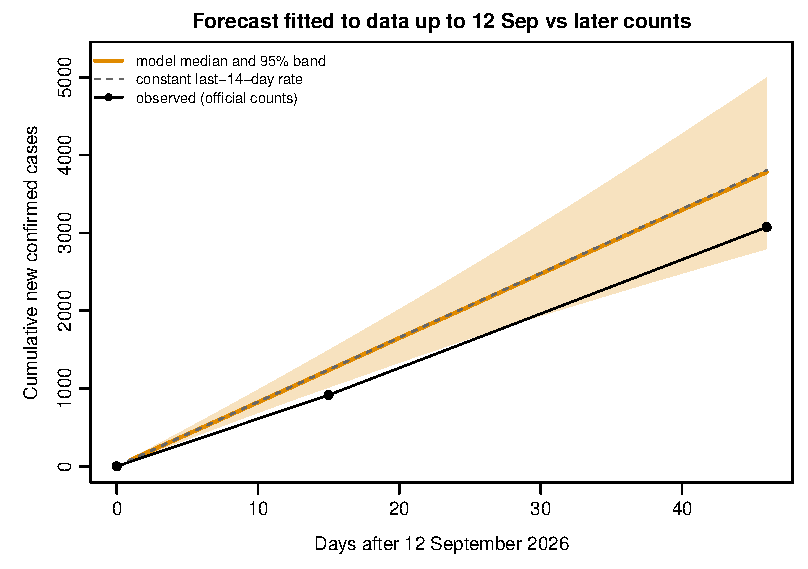
\includegraphics[width=0.62\textwidth]{fig8_validation.pdf}
\caption{Forecast of cumulative new confirmed cases after 12 September 2026 against the official counts on 27 September and 28 October.}\label{fig:val}\end{figure}

%% ======================================================================================================================
\section{Discussion}
\textbf{Principal findings.} In a model anchored to the observed course of the DRC outbreak, shortening the mean onset-to-isolation delay from 7 to 5 or 3 days turns a plateau into a decline, avoiding most of the next year's cases in every scenario tested, provided that the current delay really is about 7 days. At 80\% isolation effectiveness the reductions were \pctMedEightyFive{} and \pctMedEightyThree, $\Rt$ fell to \ReMedEightyFive{} and \ReMedEightyThree, and the median end of transmission moved from beyond five years to about \durEightyFive{} and \durEightyThree{} months. Speed and quality both matter: even a 3-day delay left \durFiftyThree{} months of transmission if isolation was only 50\% effective, and PRCC for effectiveness was nearly as large as for the delay.

\textbf{Why the effect is large, and when it would not be.} The effect on cumulative cases is large because the outbreak is close to threshold. A shorter delay raises the share of cases isolated before removal (from \aIsoSeven{} to \aIsoFive{} and \aIsoThree), which lowers $\Rt$ by a fixed proportion: from Eq.~\eqref{eq:Re}, $\Rt$ is multiplied by $(1-\epsilon a_{\text{new}})/(1-\epsilon a_{7})$ with $a=\tau/(\tau+\gamma)$. At $\epsilon=0.8$ this factor is 0.89 for a 5-day delay and 0.73 for a 3-day delay. When baseline $\Rt\approx1$ any such factor produces exponential decline; when baseline $\Rt$ is higher it does not. Table~\ref{tab:crit} gives the largest baseline $\Rt$ that each delay could bring below 1. Before the July slowdown $\Rt$ was about \fitBReBeforeMed; a 3-day delay with 80\% or better isolation would then have been sufficient (threshold \critReEightyThree), a 5-day delay would not (\critReEightyFive). Percentage reductions over 12 months should therefore not be transferred to settings or periods with a higher $\Rt$.

\begin{table}[H]\centering\small
\caption{Largest baseline reproduction number (with a 7-day delay) that a new delay can bring below 1, from Eq.~\eqref{eq:Re} with $\gamma=1/7$.}\label{tab:crit}
\begin{tabular}{@{}rcc@{}}
\toprule
Isolation effectiveness & 5-day delay & 3-day delay \\
\midrule
50\% & 1.06 & 1.15 \\
80\% & 1.13 & 1.36 \\
100\% & 1.20 & 1.67 \\
\bottomrule
\end{tabular}
\end{table}

\textbf{What ``delay'' means.} In an exponential model with competing removal, the mean delay is not the mean time to isolation of those who are isolated: with a 7-day delay and a 7-day infectious period only about half of cases are isolated at all. A field-measured onset-to-isolation or onset-to-sample delay is conditional on being isolated, so the two are not interchangeable. The structural analyses bracket this: less variable delays and the conditional definition give larger benefits (up to \varCondFive\% and \varCondThree\%), not smaller, so the base-case figures are not extreme in either direction on this point. A related point is that infectiousness of Ebola disease changes with time since onset, which the model ignores.

\textbf{Operational implications.} The results support effort aimed at shortening the delay, with the caveat that benefits depend on isolation actually preventing contact: the most effective route would combine faster detection (community alert networks, decentralised sampling, rapid result return, which the preprint puts at 8.6 days from onset to test result \citep{ebengo2026}) with isolation capacity and quality (occupancy was above 100\% in some facilities and 59\% of confirmed deaths occurred outside treatment units \citep{kabasele2026}). Gains diminish: the second two days of improvement add less than the first two. The implementation ramp-up analysis shows that a 90-day roll-out would reduce the 5-day benefit from \pctMedEightyFive{} to \varRampNinetyFive\% (lower limit \varRampNinetyUiLo\%).

\textbf{Comparison with the literature.} Our qualitative conclusion that both speed and effectiveness of isolation determine control is consistent with the Ebola review of Chowell and Nishiura \citep{chowell2014}, with earlier analyses of controllability \citep{fraser2004,lipsitch2003}, and with West African analyses linking faster isolation and community care to reduced transmission \citep{pandey2014,kucharski2015,faye2015}. Projections for the present outbreak by Mooring et al.\ varied the \emph{fraction} isolated with a 2-day delay and perfect isolation \citep{mooring2026}; ours instead varies the delay itself with imperfect isolation and is anchored to the observed surveillance. Our baseline reproduction numbers (\fitBReBeforeMed{} rising phase; \fitBReAfterMed{} plateau) are lower than the 2.5--3.5 estimates reported early in the outbreak by branching-process and spatial models \citep{mooring2026,ebengo2026}, consistent with substantial control having already occurred; they are within the 1.3--2.7 range of earlier Central African outbreaks \citep{chowell2014,lekone2006,legrand2007}.

\textbf{Strengths.} The analysis is anchored to the outbreak's own data, accounts for right-truncation and a retrospective data reconciliation, propagates fit and literature uncertainty jointly in paired scenarios, checks conclusions with a stochastic model, global and structural sensitivity analyses and an out-of-sample forecast, and is fully reproducible from raw data with unit-tested code.

\textbf{Limitations.}
(1) \emph{Delay structure.} The exponential competing-risk delay and constant infectiousness are simplifications; the structural analyses suggest conclusions are conservative in the direction tested, but infectiousness rising with time since onset, and post-mortem transmission at unsafe burials, are not modelled.
(2) \emph{Baseline delay.} The 7-day baseline is taken from the study brief and could not be confirmed in the primary source; shorter true delays would reverse the benefit of a 5-day target.
(3) \emph{Identifiability.} Case counts constrain growth, not $\epsilon$, the delay or the natural history; $\epsilon$ is a scenario assumption and the literature ranges are not drawn from the Nash database.
(4) \emph{Data.} Confirmed cases depend on testing, definitions and harmonisation; the onset curve is digitised and covers about two thirds of cases; we treated national data as homogeneous, whereas provinces differ (declining in Ituri, rising in North Kivu \citep{ukhsa2026}).
(5) \emph{Forecast error.} The out-of-sample forecast overestimated by \valErrLong{} at 46 days; absolute counts are conditional on the plateau at 12 September, although percentage effects were insensitive to starting incidence.
(6) \emph{Omitted processes.} No contact tracing, health-worker infections, spatial structure, isolation-capacity constraints, behaviour change, or changes in fatality ratio; deaths averted are illustrative.
(7) \emph{Horizon and threshold.} Percentages depend on the 12-month horizon and on baseline $\Rt\approx1$.
(8) \emph{Counterfactual timing.} Scenarios begin on 12 September; the actual course since then is only used for validation.

\textbf{Further work.} (i) Measure onset-to-isolation delays directly (line list); (ii) model the delay as a gamma-distributed waiting time with explicit isolated fraction; (iii) add contact tracing, health-care and funeral transmission; (iv) fit province-specific transmission; (v) refit with updated data to 28 October and beyond; (vi) replace literature ranges by the Nash et al.\ parameter database; (vii) add costs of delay-reduction options.

\section{Conclusion}
For a model anchored to the observed course of the 2026 BVD outbreak, reducing the mean onset-to-isolation delay from 7 to 5 or 3 days would avert most cases over the next year and bring forward the end of transmission by years, provided isolation is effective and the true current delay is about 7 days. The principal uncertainties are the true current delay, the effectiveness of isolation and the baseline growth rate, all of which can be reduced by measurement. We recommend that onset-to-isolation delay be measured and reported routinely.

\section*{Declarations}
\textbf{Author contributions.} All authors contributed equally to the project (conception, modelling, analysis and writing); individual CRediT roles to be specified by the authors.
\textbf{Funding.} None declared (to be confirmed).
\textbf{Competing interests.} None declared (to be confirmed).
\textbf{Ethics.} Only aggregated, publicly available surveillance data were used.
\textbf{Data and code availability.} Surveillance data are in \texttt{data/bvd\_2026/} (public sources, see their README); the analysis code, tests, results and this manuscript's source are in the accompanying repository; \texttt{R/run\_all.R} regenerates every number, table and figure.
\textbf{Use of generative AI.} Generative AI (Claude, Anthropic) was used for brainstorming, structuring the modelling workflow, explaining technical concepts, writing and testing analysis code, and drafting and language editing of this manuscript. The authors are responsible for reviewing and approving all analyses, interpretations and written content, and for verifying the references.
\textbf{Acknowledgements.} We thank our advisers Dr James Azam and Andrej Jarynowski, and the INSP, INRB-UMIE and BVDOutbreakSize teams whose public data made this analysis possible.

{\small\bibliographystyle{unsrtnat}\bibliography{references}}

%% ======================================================================================================================
\appendix\clearpage\nolinenumbers
\section{Mathematical details}\label{app:math}
\textbf{Reproduction number.} For Model~\eqref{eq:model} with $S=N$, one case in $I$ spends $1/(\tau+\gamma)$ days non-isolated and is isolated with probability $a=\tau/(\tau+\gamma)$, after which it spends a further $1/\gamma$ days at relative infectiousness $1-\epsilon$. Hence $\Rt=\beta\{1/(\tau+\gamma)+a(1-\epsilon)/\gamma\}=(\beta/\gamma)(1-\epsilon a)$, which is Eq.~\eqref{eq:Re} (next-generation method \citep{vandendriessche2002}).

\textbf{Erlang delay.} Replacing $I$ by $m$ stages $I_1,\dots,I_m$ with progression rate $m\tau$ and removal $\gamma$ from each, and isolation on leaving $I_m$, gives $a^m$ with $a=m\tau/(m\tau+\gamma)$ as the isolated share and $\Rt=(\beta/\gamma)(1-\epsilon a^m)$; as $m\to\infty$ the delay is fixed and the isolated share is $e^{-\gamma D}$ ($0.37$ for $D=\gamma^{-1}=7$). This is used for the Erlang-3 and Erlang-10 analyses (function \texttt{make\_rhs}).

\textbf{Calibration.} For fixed $(\sigma,\gamma,\tau_0,\epsilon)$ the growth rate of the linearised system with state $(E,I_1..I_m,Q)$ is the dominant eigenvalue of its Jacobian; $\beta$ is the root of $\text{eig}(\beta)=r$ (\texttt{uniroot}). The relation between growth rate and $\Rt$ depends on the generation-time distribution \citep{wallinga2007}, which is why $\beta$ is recalibrated per draw. In the stochastic model the same is done with the one-step expected-value matrix.

\textbf{Initial state.} The scenario starts from the dominant eigenvector (the stable distribution across $E,I,Q$ at the baseline), scaled so that $\sigma E=i(T)$ (the fitted incidence on 12 September).

\textbf{Reporting delay.} With $c(L)=1-\exp\{-((L+0.5)/s)^\kappa\}$ the daily delay probability mass is $p(L)=c(L)-c(L-1)$, $c(-1)=0$. Fit B uses expected cumulative reports $\hat C(u)=\sum_{v\le u}\sum_{d\le v}i(d)p(v-d)$ and increments $\hat C(u_j)-\hat C(u_{j-1})$ over report intervals.

\textbf{Stochastic model.} Per step $\Delta t$: $n_{SE}\sim\text{Bin}(S,1-e^{-\lambda\Delta t})$, $n_{EI}\sim\text{Bin}(E,1-e^{-\sigma\Delta t})$, $n_{IQ}\sim\text{Bin}(I,1-e^{-\tau\Delta t})$, then removals $\text{Bin}(I-n_{IQ},1-e^{-\gamma\Delta t})$ and $\text{Bin}(Q,1-e^{-\gamma\Delta t})$.

\textbf{PRCC.} Ranks of each input and of the output are regressed on the ranks of the other inputs; the PRCC is the correlation of the residuals \citep{blower1994,marino2008}.

\section{Supplementary tables}
\begin{table}[H]\centering\small\caption{Partial rank correlation of 12-month cases with each parameter.}\label{tab:prcc}\begin{tabular}{@{}lc@{}}
\toprule
Parameter (range sampled) & PRCC (95\% bootstrap CI) \\
\midrule
Isolation delay & 0.94 (0.93 to 0.94) \\
Isolation effectiveness & -0.80 (-0.82 to -0.77) \\
Baseline growth rate & 0.42 (0.38 to 0.46) \\
Latent period & 0.27 (0.21 to 0.32) \\
Starting incidence & 0.17 (0.13 to 0.21) \\
Infectious period & 0.10 (0.04 to 0.14) \\
\bottomrule
\end{tabular}
\end{table}
\begin{table}[H]\centering\small\caption{Fit B refitted at extreme natural-history values (change date fixed at the best estimate; $\epsilon=0.8$).}\label{tab:nh}\begin{tabular}{@{}cccccc@{}}
\toprule
Latent (d) & Infectious (d) & Neg.\ log-lik. & $\beta$ after & Growth rate after (/d) & Incidence 12 Sep (/d) \\
\midrule
4.0 & 5 & 407.60 & 0.300 & -0.0001 & 81.7 \\
10.1 & 5 & 407.59 & 0.298 & -0.0005 & 81.2 \\
4.0 & 10 & 407.62 & 0.191 & 0.0009 & 83.5 \\
10.1 & 10 & 407.58 & 0.190 & 0.0002 & 82.4 \\
\bottomrule
\end{tabular}
\end{table}
\begin{table}[H]\centering\small\caption{Transmission rate and reproduction number by isolation effectiveness (refit at the best change date). The growth rates, which are what the data identify, do not depend on $\epsilon$.}\label{tab:byeff}\begin{tabular}{@{}clccccc@{}}
\toprule
Fit & Isolation eff. & $\beta$ before & $\beta$ after & Growth after (/d) & $R_e$ before & $R_e$ after \\
\midrule
A & 50\% & 0.235 & 0.201 & 0.0046 & 1.24 & 1.06 \\
B & 50\% & 0.233 & 0.191 & 0.0003 & 1.23 & 1.00 \\
A & 80\% & 0.288 & 0.250 & 0.0044 & 1.21 & 1.05 \\
B & 80\% & 0.286 & 0.238 & 0.0000 & 1.20 & 1.00 \\
A & 100\% & 0.339 & 0.298 & 0.0043 & 1.19 & 1.04 \\
B & 100\% & 0.337 & 0.285 & -0.0003 & 1.18 & 1.00 \\
\bottomrule
\end{tabular}
\end{table}
\begin{table}[H]\centering\small\caption{Testing and positivity by month, 2026 (new confirmed cases after removing the 22 July step; samples analysed per day interpolated over missing days).}\label{tab:pos}\begin{tabular}{@{}lcccc@{}}
\toprule
Month (2026) & New confirmed cases & Samples analysed & Samples per day & Positivity (\%) \\
\midrule
Jun & 987 & 4,365 & 168 & 22.6 \\
Jul & 1,996 & 9,102 & 294 & 21.9 \\
Aug & 2,512 & 13,373 & 431 & 18.8 \\
Sep & 1,014 & 5,927 & 494 & 17.1 \\
\bottomrule
\end{tabular}
\end{table}

\section{Repository layout and how to reproduce}\label{app:repro}
\small
\begin{verbatim}
taus-isolation-delay/
  README.md              how to run; run times; caveats
  data/
    bvd_2026/            surveillance streams (public; its README states sources and caveats)
    cumulative_confirmed_drc.csv   later official counts used only for validation
  R/
    00_functions.R       model, calibration, stochastic engine, helpers, constants (CFG)
    01_data_prep.R       reporting delay and the two fitting datasets
    02_fit.R             maximum likelihood fit, profile over change date, draws, adequacy
    03_scenarios.R       nine scenarios x paired draws; policy surface
    04_stochastic.R      stochastic check
    05_sensitivity.R     PRCC and structural variants
    06_validation.R      out-of-sample forecast
    07_figures_tables.R  figures, LaTeX tables, number macros (manuscript/numbers.tex)
    run_all.R            runs tests, scripts 01-07, then compiles the manuscript
  tests/test_model.R     unit tests of the model code
  manuscript/            main.tex, references.bib, numbers.tex (auto-generated)
  results/, figures/     all outputs (regenerated)
\end{verbatim}
\textbf{To reproduce:} install R (here \rVersion) and the \texttt{deSolve} package, then run \texttt{Rscript R/run\_all.R} from the repository root (about 15 minutes) and, to rebuild the PDF, \texttt{pdflatex}/\texttt{bibtex} in \texttt{manuscript/}. Random seeds are set at the top of each script. The test script must pass before any analysis is run.
\normalsize

\section{R code}\label{app:code}
The scripts below are inserted directly from the repository files so the listing always matches the analysis. (\texttt{R/07\_figures\_tables.R}, which only draws figures and writes tables and macros, and \texttt{R/run\_all.R} are in the repository.)
\subsection*{R/00\_functions.R}\lstinputlisting{../R/00_functions.R}
\subsection*{R/01\_data\_prep.R}\lstinputlisting{../R/01_data_prep.R}
\subsection*{R/02\_fit.R}\lstinputlisting{../R/02_fit.R}
\subsection*{R/03\_scenarios.R}\lstinputlisting{../R/03_scenarios.R}
\subsection*{R/04\_stochastic.R}\lstinputlisting{../R/04_stochastic.R}
\subsection*{R/05\_sensitivity.R}\lstinputlisting{../R/05_sensitivity.R}
\subsection*{R/06\_validation.R}\lstinputlisting{../R/06_validation.R}
\subsection*{tests/test\_model.R}\lstinputlisting{../tests/test_model.R}
\end{document}
